\documentclass{article}

\usepackage{graphicx}
\usepackage{float}

\begin{document}

Given the parameters for a perspective projection we want to find a corresponding orthographic projection matrix and vice versa. The target projection should include the exact same portion of a plane perpendicular to the view direction. The plane is given by the distance to the camera.
The following text explains the computation from perspective to orthographc. The other way is handled analogously.

A perspective projection is specified by a field of view, the aspect ratio and the distance to the near-/far plane ($zNear, zFar$). As opposed to a orthographic projection, which usually takes the distances of the edges to the center of the near plane as input.
This leaves us with two tasks:
\begin{enumerate}
  \item{convert field of view and aspect ratio ($fovy, ar$) to left, right, top, bottom ($l_p,r_p,b_p,t_p$)}
  \item{transform left, right, top, bottom to find the orthographic bounds ($l_o,r_o,b_o,t_o$)}
\end{enumerate}

To convert field of view and aspect ratio we use some simple trigonometrie. Figure~\ref{fig:fovyConversion} visualizes the given situation for the right bound, $r_p$ we are looking for.
\begin{figure}[H]
  \centering
  \label{fig:fovyConversion}
  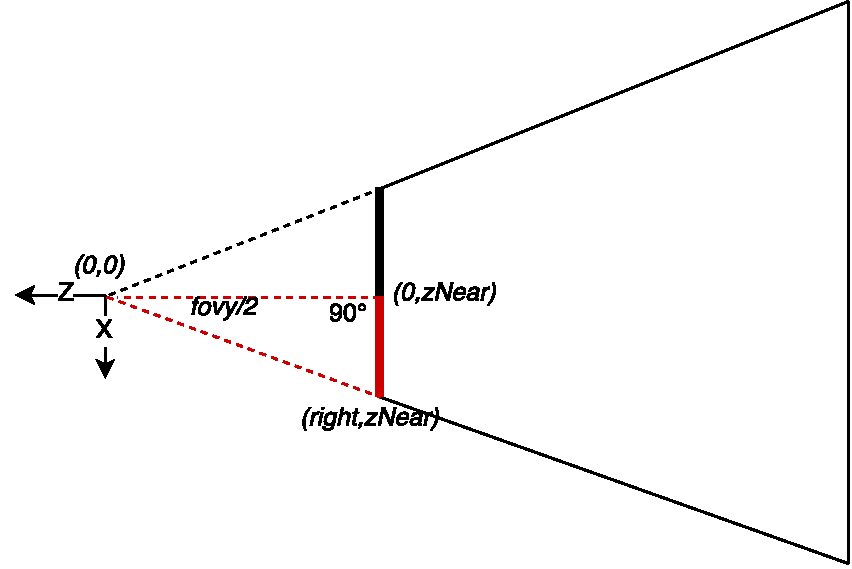
\includegraphics[width=0.8\textwidth]{fovyConversion}
  \caption{The red triangle is used to compute $r_p$}
\end{figure}

We have the angle $fovy/2$, the length of the adjacent, which is $zNear$, and are looking for the length of the opposite, right side ($r_p$). The tangent results in the following equation:
\begin{equation}
 \tan{(fovy/2)} = \frac{r_p}{zNear}\qquad
 r_p = zNear*\tan{(fovy/2)}
\end{equation}
We can compute $l_p$ the same way or just assume that the frustrum is symmetric. $t_p, b_p$ result from the aspect ratio. In the symmetric case we take $ar=2r_p/2t_p$, solve for $t_p$ and we get $t_p=r_p/ar$.

As the second step $l_p,r_p,b_p,t_p$ are translated along the inverse z-axis up to the point of syncronisation and are used as input for the new orthographic projection. This is visualized in figure~\ref{fig:projections}.

\begin{figure}[H]
  \centering
  \label{fig:projections}
  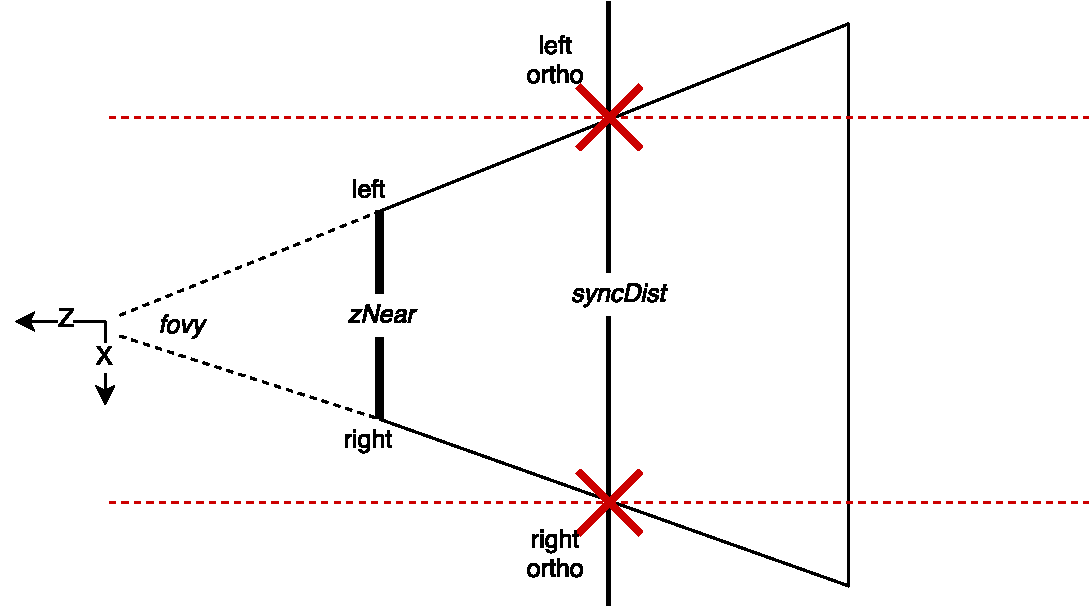
\includegraphics[width=0.8\textwidth]{projections}
  \caption{Top view of perspective projection}
\end{figure}

During construction of a perspective projection, a point in eye space is projected on the near plane using the ratio of similar triangles. For the x coordinate ($x_e$) it looks like this; note that here $z_e$ is negative, thus the $-zNear$:
\begin{equation}
    \frac{x_p}{x_e} = \frac{-zNear}{z_e}\qquad
    x_p = \frac{zNear*x_e}{-z_e}
\end{equation}

We can use this equation since we want the reverse translation for the most outer values. Therefore we set $x_e$ to $r_o$, $x_p$ to $r_p$, $z_e$ to $-syncDist$ (since this is positive in contrast to $z_e$), and solve for $r_o$.
\begin{equation}
    \frac{r_p}{r_o} = \frac{-zNear}{-syncDist}\qquad
    r_o = \frac{r_p*syncDist}{zNear}
\end{equation}

This is done only for right and top, because we assume a symmetric view frustrum. Hence, $r_o = -l_o$ and $-b_o = t_o$.










\end{document}
